\documentclass[10pt]{beamer}
\usepackage{graphicx}
\usepackage{adjustbox}
\usepackage{hyperref}

\usetheme{Copenhagen}
\usecolortheme{seagull}  % You can choose from various color themes provided by metropolis
% \setbeamertemplate{footline}[frame number]
\setbeamertemplate{navigation symbols}{}

\title[WP1]{
  
\includegraphics[width=0.8\textwidth]{images/logo_Uni.png}
  Project WP1 - Vegetation}
\author[SCP]{Giulio CARPI LAPI, Pierre-Antoine SENGER}

\begin{document}

\frame{\titlepage}

\begin{frame}{Impact of vegetation on urban heat}
  \begin{figure}[h] % 'h' option tries to place the figure here
    \centering
    \includegraphics[width=1\textwidth]{images/heat_street.png}
    \caption{thermal signature of a street \cite{street_thermography}} % Caption for referencing
    \label{fig:heat_street} % Label for referencing
  \end{figure}
\end{frame}

\begin{frame}{Aerial thermography}
  \begin{figure}[h] % 'h' option tries to place the figure here
    \centering
    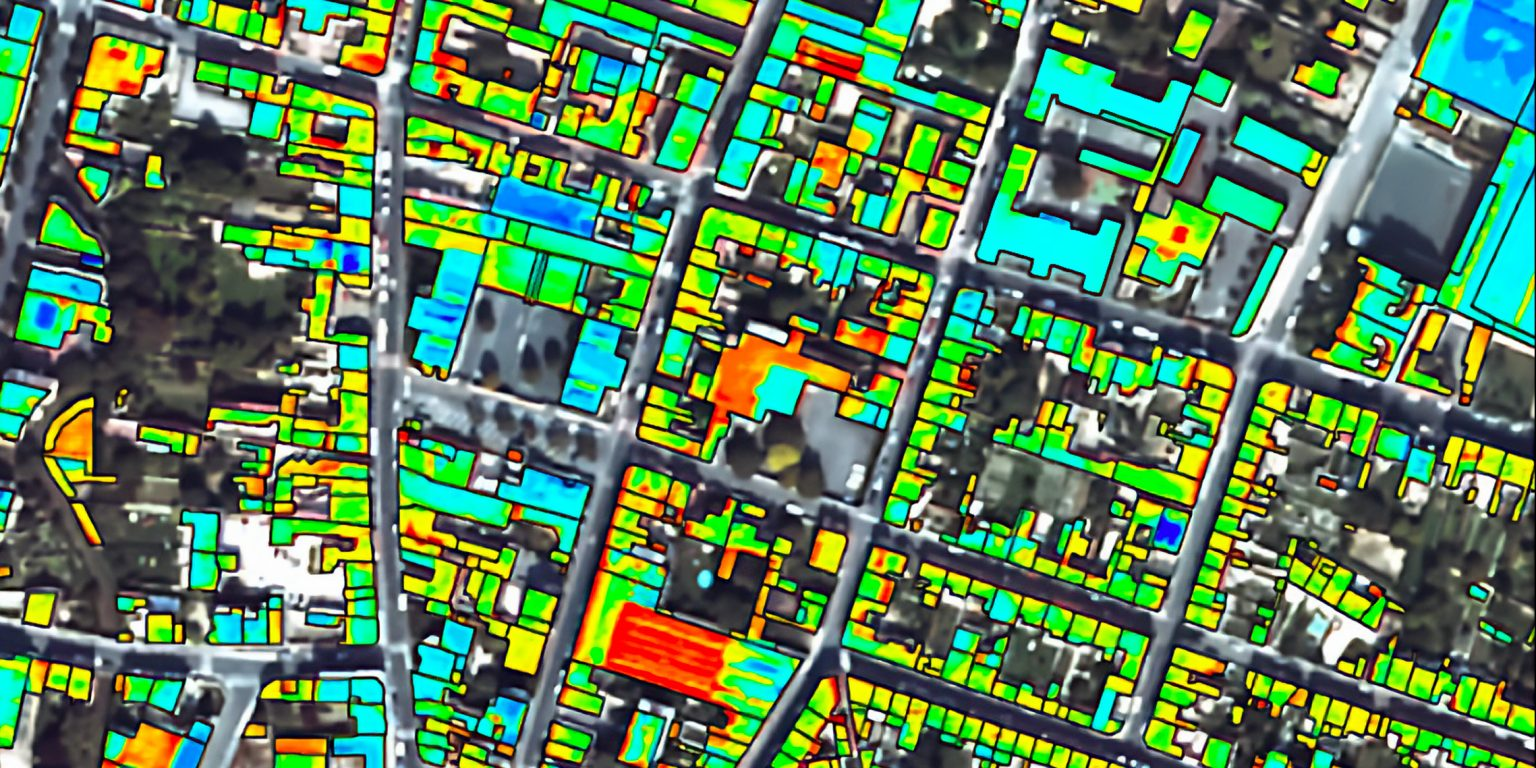
\includegraphics[width=1\textwidth]{images/thermographie-aerienne.jpg}
    \caption{aerial thermography of a city \cite{thermography}} % Caption for referencing
    \label{fig:thermographie} % Label for referencing
  \end{figure}
\end{frame}

\begin{frame}{3D city model}
  \begin{figure}[h] % 'h' option tries to place the figure here
    \centering
    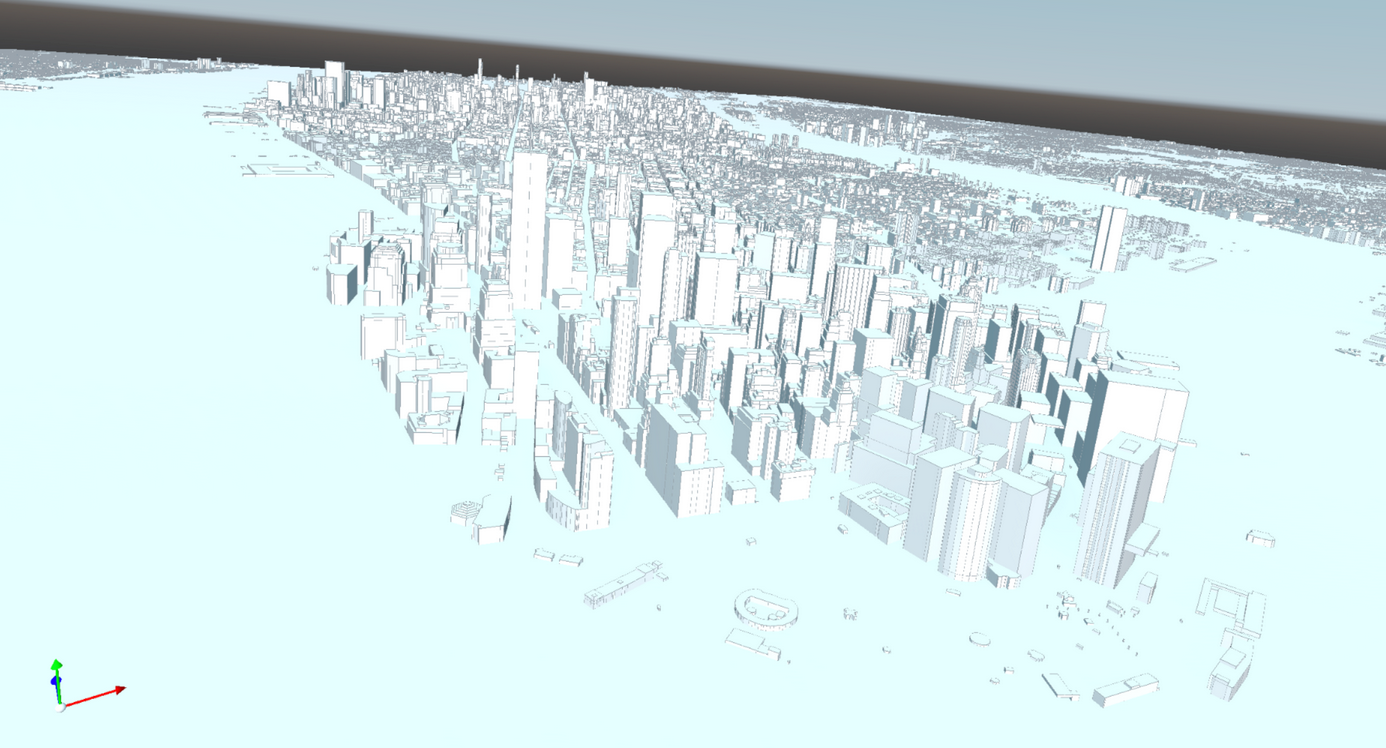
\includegraphics[width=1\textwidth]{images/NY_mesh.png}
    \caption{3D city model of New York \cite{NY-mesh}} % Caption for referencing
    \label{fig:3d_city_model} % Label for referencing
  \end{figure} % This was missing
\end{frame}

\begin{frame}{Objectives}
  \begin{itemize}
    \item<1-> Access the OpenStreetMap database to extract metadata \\
    (location, height, species, etc.)
    \item<2-> Create a 3D models library of trees
    \item<3-> Integrate the 3D trees in the 3D city model
    \item<4-> Run simulations
  \end{itemize}
\end{frame}

\begin{frame}{Roadmap V0}
  \begin{figure}[h] % 'h' option tries to place the figure here
    \centering
    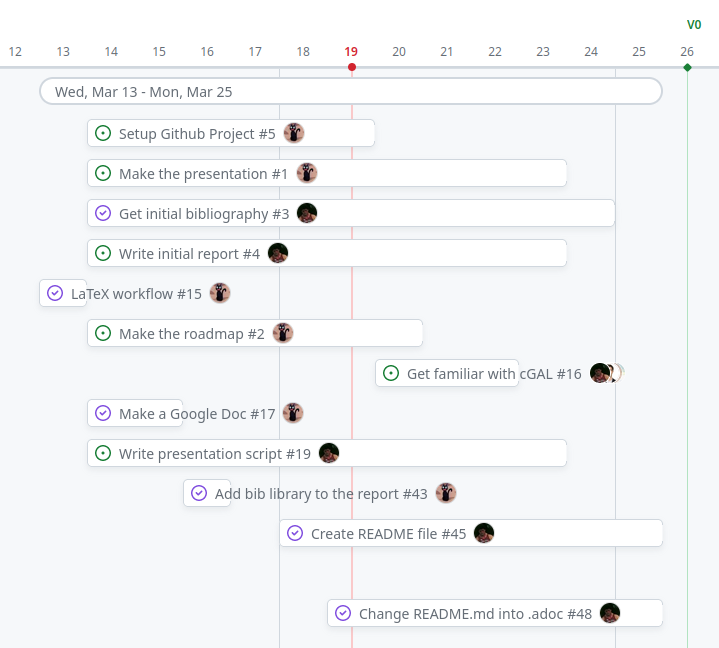
\includegraphics[width=0.8\textwidth]{images/roadmap_v0.png}
    \caption{Roadmap V0} % Caption for referencing
    \label{fig:roadmap_v0} % Label for referencing
    \end{figure}
\end{frame}

\begin{frame}{Roadmap V1}
  \begin{figure}[h] % 'h' option tries to place the figure here
    \centering
    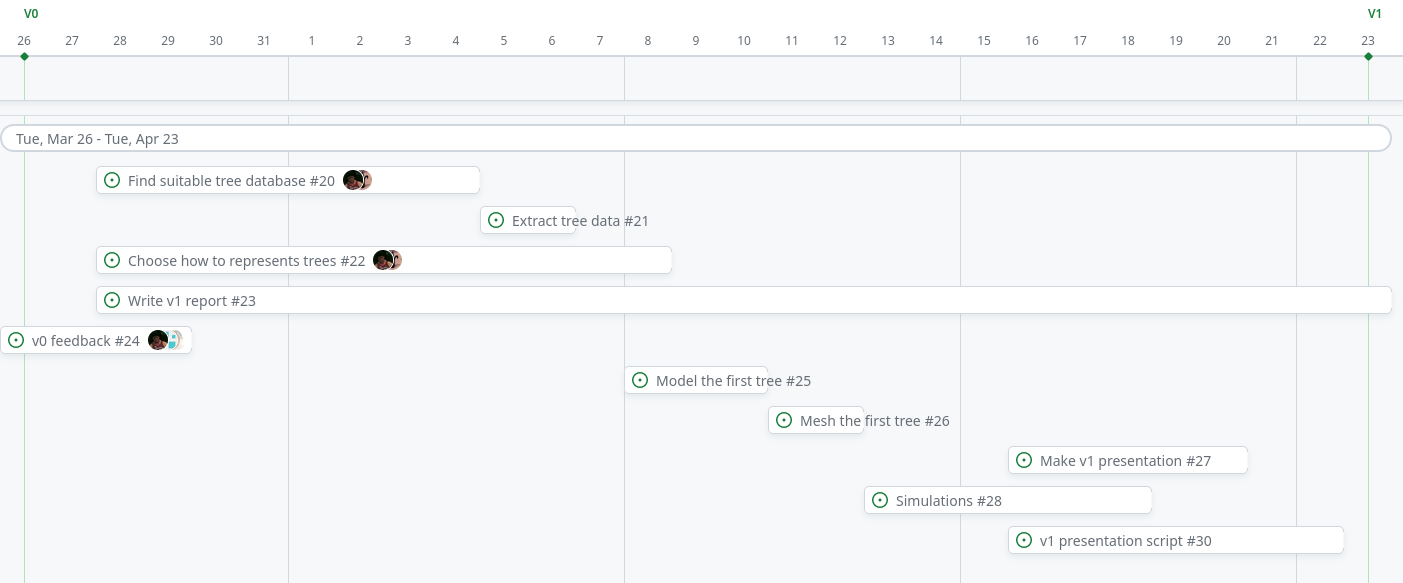
\includegraphics[width=1\textwidth]{images/roadmap_v1.png}
    \caption{Roadmap V1} % Caption for referencing
    \label{fig:roadmap_v1} % Label for referencing
    \end{figure}
\end{frame}

\begin{frame}{Roadmap V2}
  \begin{figure}[h] % 'h' option tries to place the figure here
    \centering
    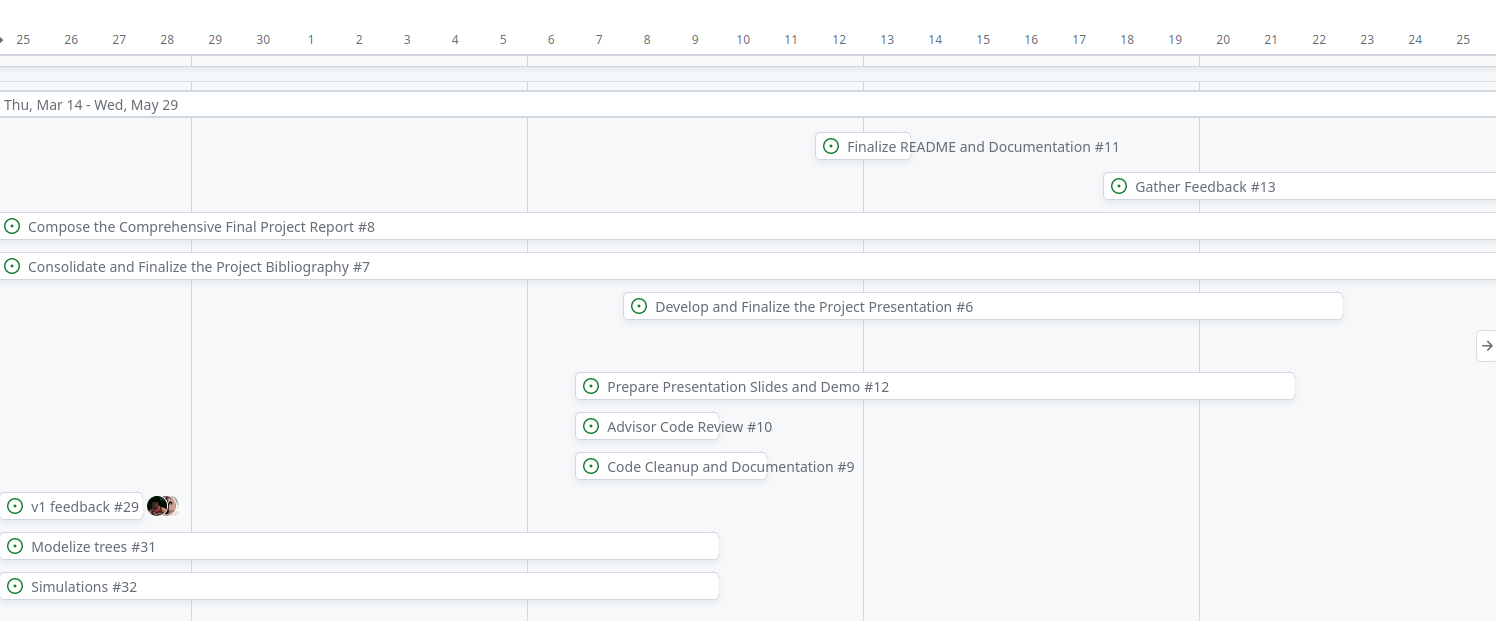
\includegraphics[width=1\textwidth]{images/roadmap_v2.png}
    \caption{Roadmap V2} % Caption for referencing
    \label{fig:roadmap_v2} % Label for referencing
    \end{figure}
\end{frame}



\begin{frame}{References}
\begin{thebibliography}{9}
  \bibitem{NY-mesh} \url{https://github.com/orgs/feelpp/discussions/2188}
  \bibitem{thermography} \url{https://www.somme.fr/services/appui-aux-collectivites/les-aides-du-departement/fonds-thermographie-aerienne/}
  \bibitem{street_thermography} \url{https://theconversation.com/dou-vient-le-pouvoir-rafraichissant-des-arbres-en-ville-199906}
  \bibitem{osm-queries} \url{https://osm-queries.ldodds.com/tutorial}
  \bibitem{osm-learnoverpass} \url{https://osmlab.github.io/learnoverpass//en/}
\end{thebibliography}
\end{frame}

\end{document}